\chapter{Introduction}\label{ch_intro}
\chapterauthor{Jeff Yoshimi, Zo\"e Tosi}{.7,.3}

% Change most italics to glossary items
% Consider changing some of the Simbrain pictures so that the size of the weights is more evident, since that is now discussed
% Maybe use some of the blue brain / human brain project pics. They are amazing.
% Need terminology for input and output to a specific weight layer. Comes up in backprop for example


% Sometimes "network" in biology also refers to networks of _brain areas_. See ch. 3
The phrase ``neural network'' has several meanings. A \glossary{biological neural network} is an actual set of interconnected neurons in an animal brain. Fig. \ref{introNets} (left) shows a biological neural network. ``Neural network'' can also mean \glossary{artificial neural network} (or ``ANN"),  that is, a computer model that has certain things in common with biological neural networks. Fig. \ref{introNets} (right) shows an artificial neural network. It has ``nodes'' and ``weights'' that are analogous to the neurons and synapses of a biological neural network. We focus on artificial neural networks in this book, and when we refer to ``neural networks'' we usually mean artificial neural networks.
% There are other ways referring to artificial neural networks, including: ``connectionist network,' or' ``PDP (parallel distributed processing) network. These differ slightly but will be treated as synonyms in what follows.

\begin{figure}[h]
\centering
\raisebox{-0.5\height}{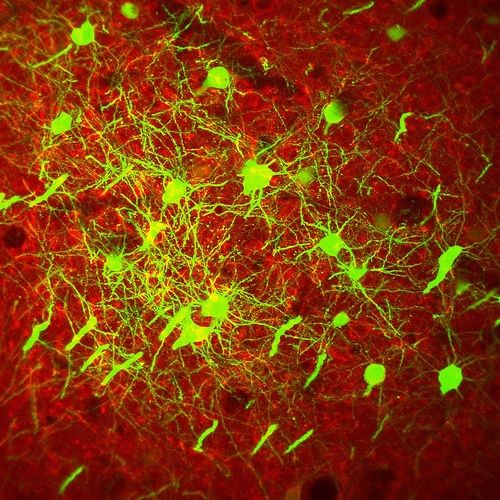
\includegraphics[scale=.3]{./images/NeuroNet.jpg}}
\hspace*{.2in}
\raisebox{-0.5\height}{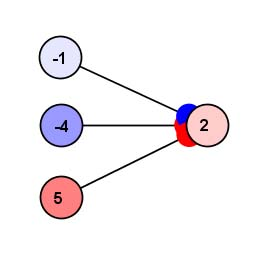
\includegraphics[scale=.5]{./images/Simple3.jpg}}
\caption[Left: Mark Miller, Nelson Lab, Brandeis University. Licensed Under: CC BY-ND; Right: Simbrain screenshot.]{Left: A biological neural network. Right: A simple artificial neural network built in Simbrain, with three nodes connecting to another node via three weights.}
\label{introNets}
\end{figure}

Neural networks can be made to do many fascinating things. They can, for example, drive cars, forecast weather patterns, recognize faces in images, and play the game Go at championship levels. Recently, they have become eerily good at producing human-level written text and images (see the discussion of GPT-3 in chapter \extref{ch_supervised_recurrent} or search the web for images produced by Dall-E). They have been used to model the brain at all of its levels, from individual neurons up to the entire brain. They have been used to model cognition in all of its forms, including memory, perception, categorization, language, and attention. In this chapter, we give a general introduction to neural networks, and survey some of these different ways they are used.\footnote{Some time in the 2010s or 2020s, it became standard to refer to neural networks as a form of ``AI'' or "Artificial Intelligence.''  From this standpoint, ``AI'' is a covering term that includes all the many forms of computer simulation that attempt to behave in an intelligent and often human-like manner.  In the earlier literature ``AI'' was used to refer to more classical, symbolic forms of artificially intelligent system, and in that era there was a kind of battle between AI and neural networks. Some of this history is covered in section \extref{cog_rev}.  The term ``AI'' is mostly avoided in this text.}

\section{Structure of Neural Networks}\label{structureNets}

In figure \ref{nodesWeights} a simple neural network is shown with some of its parts labeled. In this section, we review the parts of neural networks (nodes and weights), the ways they can be structured (their topology), and the relationship between a network and its environment. In each case, bear in mind that what precisely the concepts mean depends on the type of model we are dealing with.\footnote{Neural networks can be used for engineering, to model the brain, or to model the mind. These different uses are discussed in section \ref{typesOfResearch}. Depending on the way a network is being used, the way its parts are interpreted differs, as we'll see.} 

\begin{figure}[h]
\centering
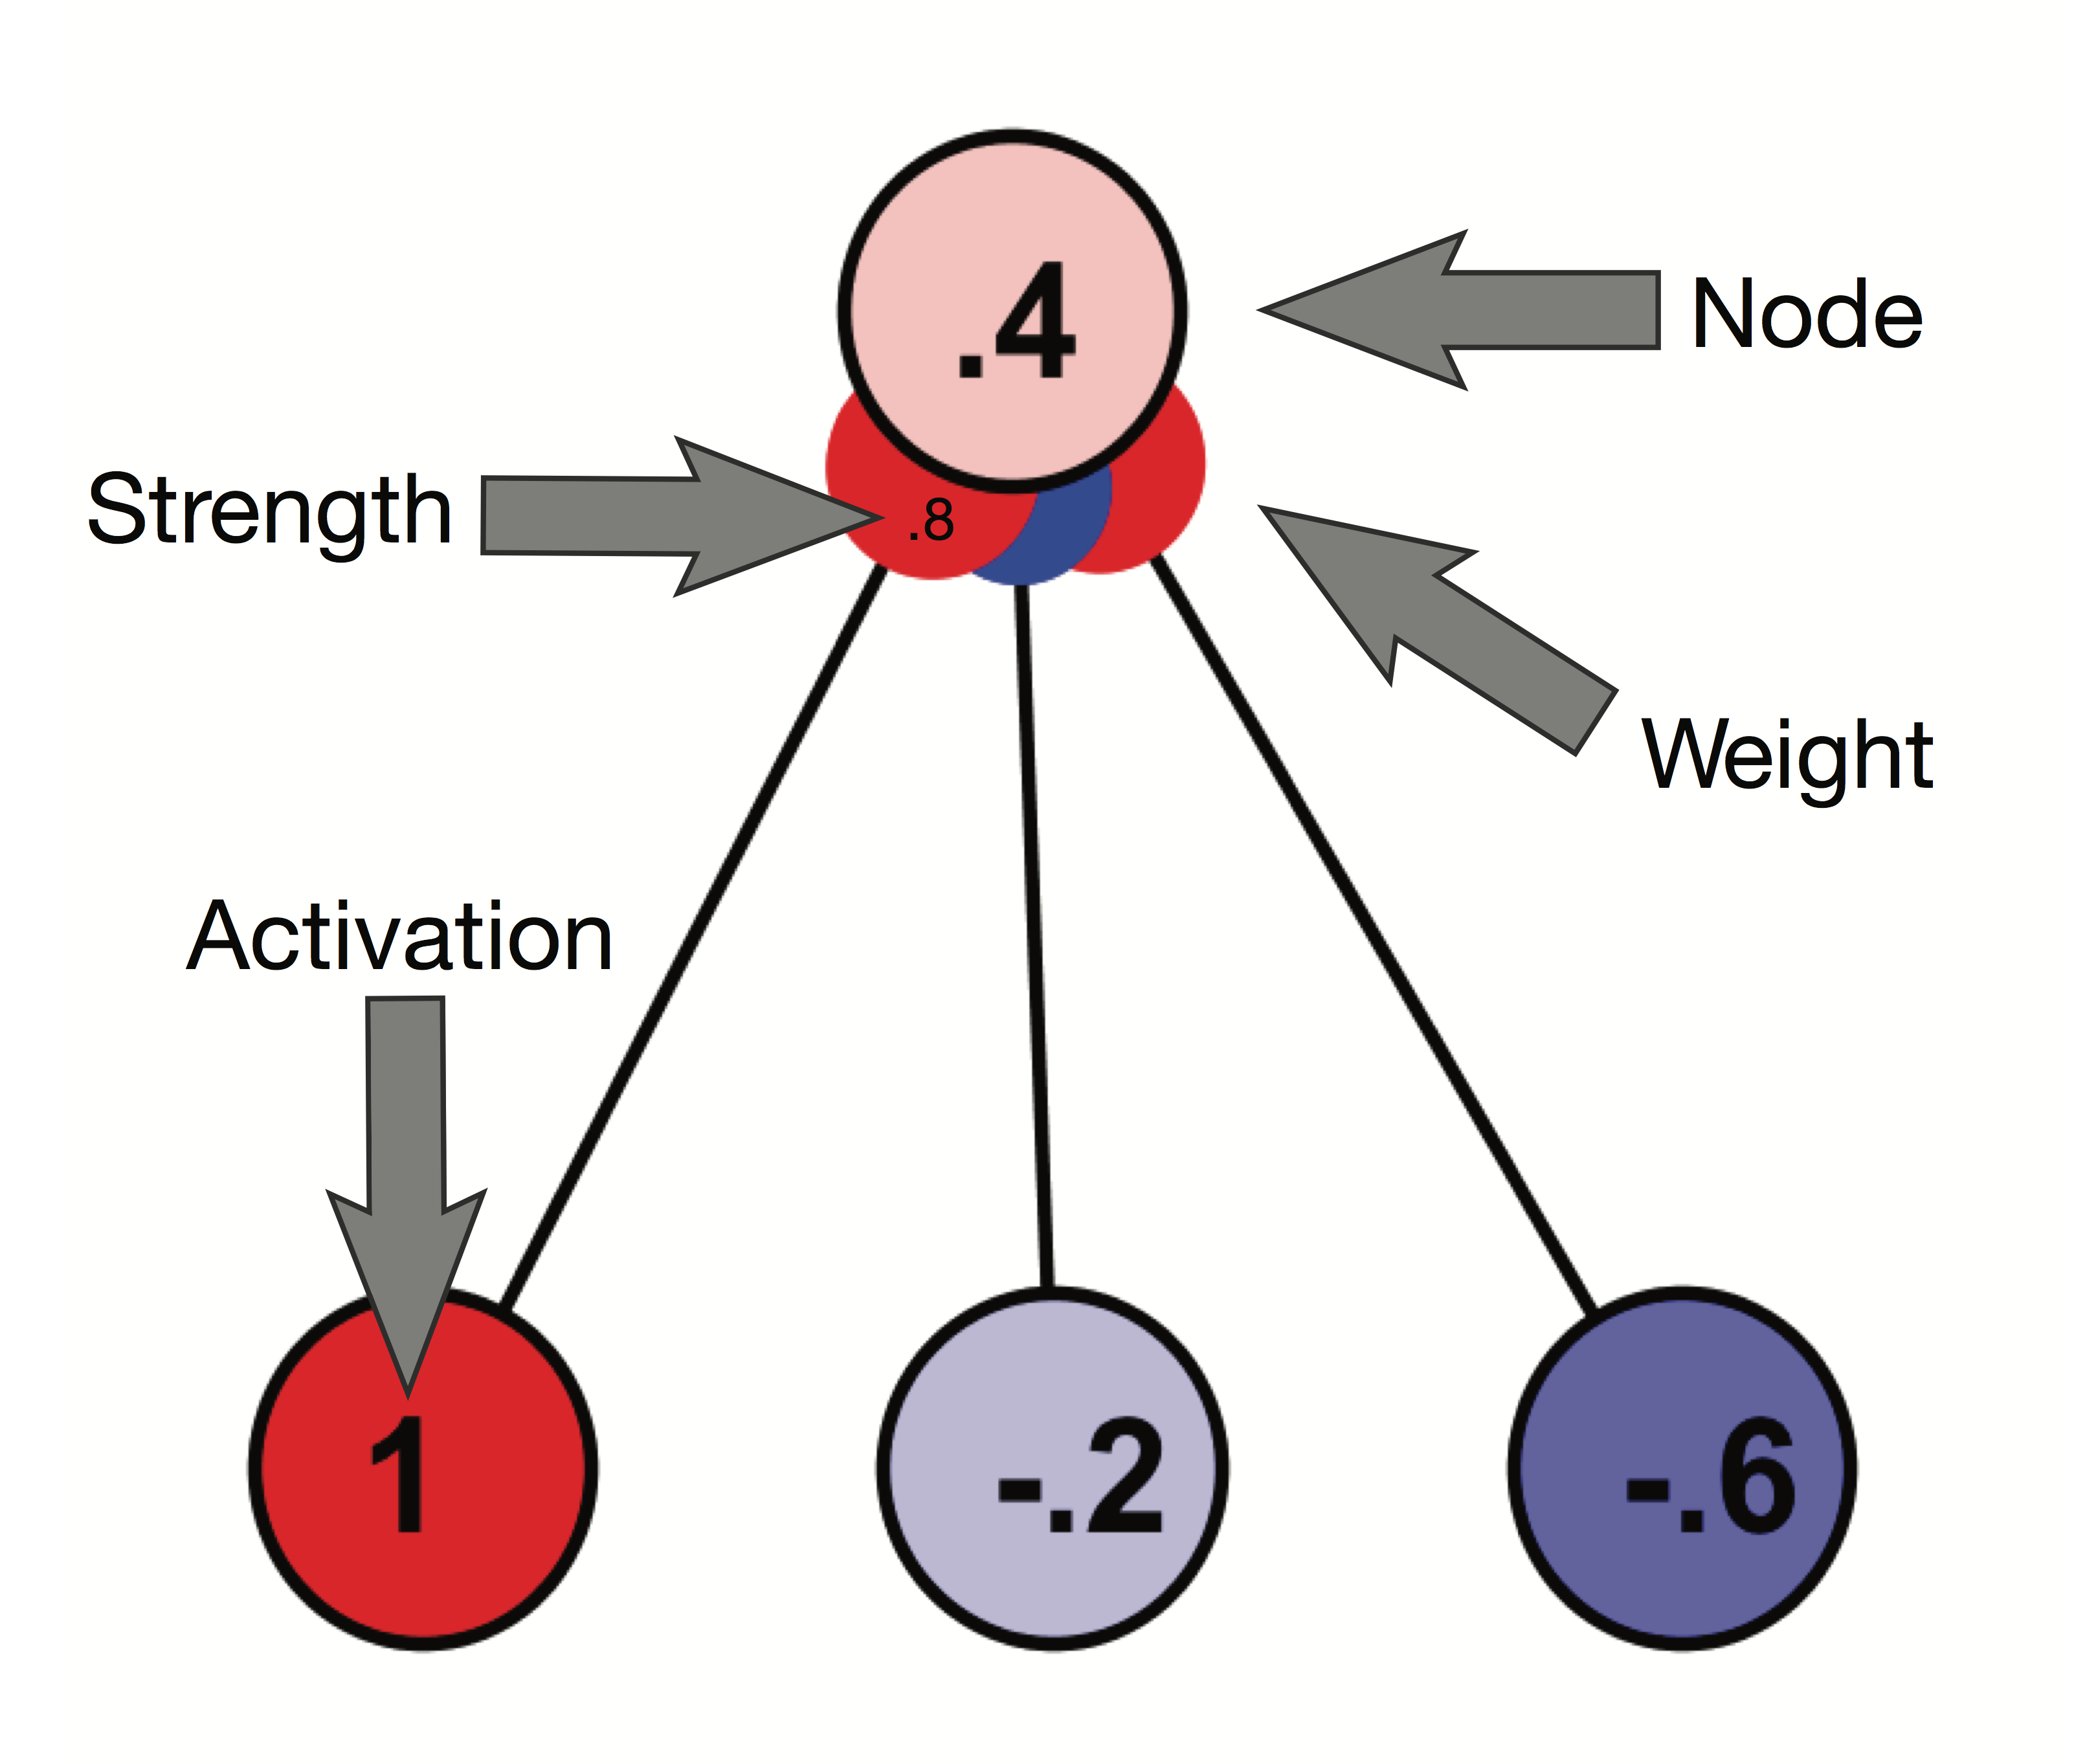
\includegraphics[scale=.2]{./images/labelledNet.png}
\caption[Simbrain screenshot with additional elements added by Pamela Payne.]{Nodes and their activations; weights and their strengths.}
\label{nodesWeights}
\end{figure}

In the figure, a circle with a number in it is an artificial neuron or \glossary{node} (nodes are also referred to as ``units'').\footnote{Sometimes, when the context makes it clear that we are talking about an artificial neural network, terms like ``neuron'' and ``synapse'' are used to mean artificial neuron (i.e. node) or artificial synapse (i.e. weight).}  The number inside a circle corresponds to that node's \glossary{activation}. In Simbrain, red corresponds to an ``active'' neuron (activation greater than 0), and how deep the red is corresponds to how close the activation is to its maximum value. Blue corresponds to an ``inhibited'' neuron (activation less than 0), and how deep the blue is corresponds to how close the activation is to its minimum value. White corresponds to an inactive neuron (activation equals 0). In a computational neuroscience model, these activations might represent the firing rate or membrane potential of a real neuron. In a psychological model, the number might represent the presence of an item in working memory, or the strength of an unconscious belief. As we will see, there is a great deal of variance in what concepts such as activation are taken to mean.
%In computational neuroscience, the numbers represent real properties of neurons and synapses. For example, in some models activation represents a firing rate (number of spikes per second), and in other models it represents a voltage. Weight strength in such models represents the efficacy of a synapse in transmitting information from one neuron to another. In connectionist models of psychological data, the interpretation of activation and weight strength is more abstract. Node activations are sometimes taken to represent the overall activity of a whole population of neurons in some region of the brain, something abstract like the ``strength of a hypothesis'', and they are sometimes simply taken to be hidden variables that have no biological significance whatsoever. \footnote{As McLelland, Rummelhart, and Hinton put it: ``These models assume that information processing takes place through the interactions of a large number of simple processing elements called units, each sending excitatory and inhibitory signals to other units. In some cases, the units stand for possible hypotheses about such things as the letters in a particular display or the syntactic roles of the words in a particular sentence. In these cases, the activations stand roughly for the strengths associated with the different possible hypotheses, and the interconnections among the units stand for the constraints the system knows to exist between the hypotheses. In other cases the units stand for possible goals and actions... and the connections relate goals to subgoals, subgoals to actions, and actions to muscle movements. In still other cases, units stand not for particular hypotheses or goals, but for aspects of these things'' \cite{mcclelland1986appeal}. Or again, as Sejnowski and Rosenberg say: ``The processing units in a network model share some of the properties of real neurons, but they need not be identified with processing at the level of single neurons. For example, a processing unit might be identified with a group of neurons, such as a column of neurons'' (Sejnowski and Rosenberg, p. 146) \cite{sejnowski1987parallel}.}
%  From Cohen et. al on Fear: "Processing units: Simple, nonlinear summing devices can be used as a first approximation of the behavior of populations of real neurons that redundantly code for the same piece of information."
% Perhaps the best discussion of this issues is in Smolensky PTC. (Around table 1)

The lines with filled disks at the end of them are artificial synaptic connections or \glossary{weight}s. These correspond to connections between nodes, which control how activation flows through a network. The weights have a value, a \glossary{strength}. The larger the absolute value of a weight strength, the ``stronger'' it is.  2 is a stronger positive weight than 1 is, and -2 is a stronger negative weight than -1 is. Thus, to strengthen a weight is to increase its absolute value, and to weaken it is to reduce its absolute value.  Stronger weights are shown as larger disks in Simbrain. The actual weight strength can be seen by hovering over the weights or double clicking on them.  As activation flows through a network, the weights with a positive strength (the red weights in Simbrain) tend to enhance activation, and the weights with a negative strength (the blue weights) tend to reduce activation.\footnote{For more details on the graphic representation see \url{http://www.simbrain.net/Documentation/docs/Pages/Network/visualConventions.html}.} In neuroscience terms, these correspond to excitatory and inhibitory synapses. As you play with simulations in Simbrain and study the chapters to come, you will begin to get a feel for how different kinds of weights have different kinds of impacts on the flow of activation in a network. 

What weight strength represents depends on what kind of model we are dealing with (see section \ref{typesOfResearch}). In a computational neuroscience model, it would represent \glossary{synaptic efficacy}--roughly speaking the impact a pre-synaptic neuron can have on a post-synaptic neuron after the pre-synaptic neuron fires an action potential. In a connectionist or psychological model, the strength might represent an association between concepts. In a machine learning model, there might be no direct interpretation of weight strengths at all: they are mere parameters in a statistical model that does something useful, like recognize faces in images.

Node activations change in accordance with \emph{activation functions} (discussed in chapter \extref{ch_act_functions}), and weight strengths change in accordance with different types of learning algorithms discussed throughout the book. Indeed, how to train neural networks is one of the most fundamental topics in the field, and is the focus of several chapters, including chapters \extref{ch_unsupervised}, \extref{ch_supervised} and \extref{ch_lms_backprop}. 

In some models a node can also produce a \glossary{spike}, which is a discrete event that corresponds to the action potential of a neuron.\footnote{A spike is represented in Simbrain by a node and all its outgoing connections turning yellow. For an illustration of a spiking node and how it looks in Simbrain, see \url{http://www.simbrain.net/Documentation/docs/Pages/Network/neuron.html}.}  Spiking neurons have their own rules and structures, which we discuss in chapter \extref{ch_spiking}.

Nodes and weights are the basic parts of a neural network. Together, they form a network structure or mathematically, a graph\footnote{\url{https://en.wikipedia.org/wiki/Graph_(discrete_mathematics)}.}, where the nodes correspond to vertices, and the weights correspond to edges.\footnote{A neural network is a special type of graph: a vertex-labeled, edge-labeled, directed graph. This means that the edges between nodes have a direction (the graph is \emph{directed}), and that numbers are associated with the vertices and edges (it is \emph{vertex-labeled} and \emph{edge-labeled}).}  The graph-structure formed by a network's nodes and weights is the network's \glossary{topology}. At a first pass, neural network topologies fall into one of two rough types shown in Fig. \ref{nn_types}: feed-forward and recurrent. We first 

% Another issue with layer concept. Sometimes it refers just to activations, sometimes to activations and all the hyperparameters, rules, etc. (i.e. what would show up in a property editor if you double clicked.)
% Are pools of IAC node layers?
% See deep leaning chapter and convolutional layers and cohere with that. Feature maps are a kind of node layer (a tensor) and convolutional layers are a special kind of weight layer.
A  \glossary{feed-forward network} is a sequence of \emph{layers} of unconnected neurons stacked on top of each other such that each layer is fully connected to the next one in the sequence (each node in one layer sends a connection to every node in the next layer).\footnote{\label{acyclic} In graph-theoretic terms, such a network is a directed, acyclic, multipartite graph. It is is \emph{acyclic} because there are no \emph{cycles}; there is is no way to ``move'' from one vertex back to itself along a sequence of vertices connected by edges. It is \emph{multi-partite} because the vertices can be partitioned into \emph{independent sets} (node layers), within which none of the vertices are connected. When such a network is not fully-connected from one layer to the next, it is still often referred to as ``feed-forward''. In some cases weights skip over a layer (e.g. go straight from input to output despite the presence of a hidden layer) and again, since activity will still flow ``forward'', this will be referred to as a feed-forward network.}  Activity in this kind of network flows from an \emph{input layer} through a sequence of \emph{hidden layers}, and then to an \emph{output layer}. Sometimes there are no hidden layers and we have a feed-forward network that connects directly from an input layer to an output layer.

% TODO: Forward references
 In a feed-forward network activity simply passes through the node layers; when activation is added to the input nodes and the network is updated, that activation flows from layer to layer and is then erased. Feed-forward networks are often classifiers: an input (which might represent an image, or a smell) passes through the layers of the network and the output activations then represent a way of classifying the input (saying who is in the image, or what object is being smelled).

% Also a link to overfitting?
In a feed-forward network we can distinguish between a \glossary{node layer} and a \glossary{weight layer}.\footnote{The distinctions introduced in this paragraph and the next one are stipulations made to organize the material in a coherent way. Terms like node layer, weight layer are not standard, but help organize the material in this book.}  We will take node layers in a feedforward network to be collections of nodes that are treated as a group, and weight layers to be collections of weights that connect node layers. Often these are represented using vectors and matrices, respectively (see chapter \extref{ch_linear_algebra}). The network in Fig. \ref{nn_types} has three node layers (labelled ``input layer'', ``hidden layer'', and ``output layer'') and two weight layers (labelled ``1-2'' and ``2-3'').\footnote{To make matters even more confusing sometimes the input node layer is \emph{not} counted as a layer.} When used without qualification, we use the term ``layer'' to mean ``node layer''.\footnote{In Simbrain, node and weight layers are both represented as groups, indicated by the yellow interaction boxes: \url{http://www.simbrain.net/Documentation/docs/Pages/Network/groups.html}.}

% Add link to universal approximator thing once we have it
We can also distinguish between the `` representational depth'' and `` representational width'' of a feed-forward network.  We take the \glossary{representational depth} of network to correspond to how many layers or layer-like structures the network has. Thus a ``deep'' network is one with many node and weight layers. The \glossary{ representational width} of a given node layer corresponds to how many nodes it has.\footnote{While the concept of depth is fairly common, ``width'' as a named concept is not. Be aware that ``width'' and ``depth'' are also used to refer to the shapes of tensors (see section \extref{sect_tensors}) but the meaning is different there, and we assume our meaning is clear in context (for example, we sometimes add ``representational'' to make it clear we mean these concepts, and not tensor shape concepts).} We will see throughout the book that these two concepts provide distinct ways of understanding the representational capacities of neural networks. A wider layer can develop more sophisticated representations of its inputs. A network with more depth can develop representations that combine features of other representations, so that we get increasingly complex ``representations of representations.'' The layers of a network trained to recognized images can go from representing lines, to sets of lines (that is, shapes), to sets of shapes, etc (see the discussion of Selfridge in chapter \extref{ch_history}, and of convolutional networks in chapter \extref{ch_cnn}). Analogues of these intuitive concepts of depth and width persist in more complex types of networks, like transformers (chapter \extref{ch_transformers}), where we can contrast the number of heads in a given block (width) with the number of blocks that are stacked on top of each other (depth). 
 
\begin{figure}[h]
\centering
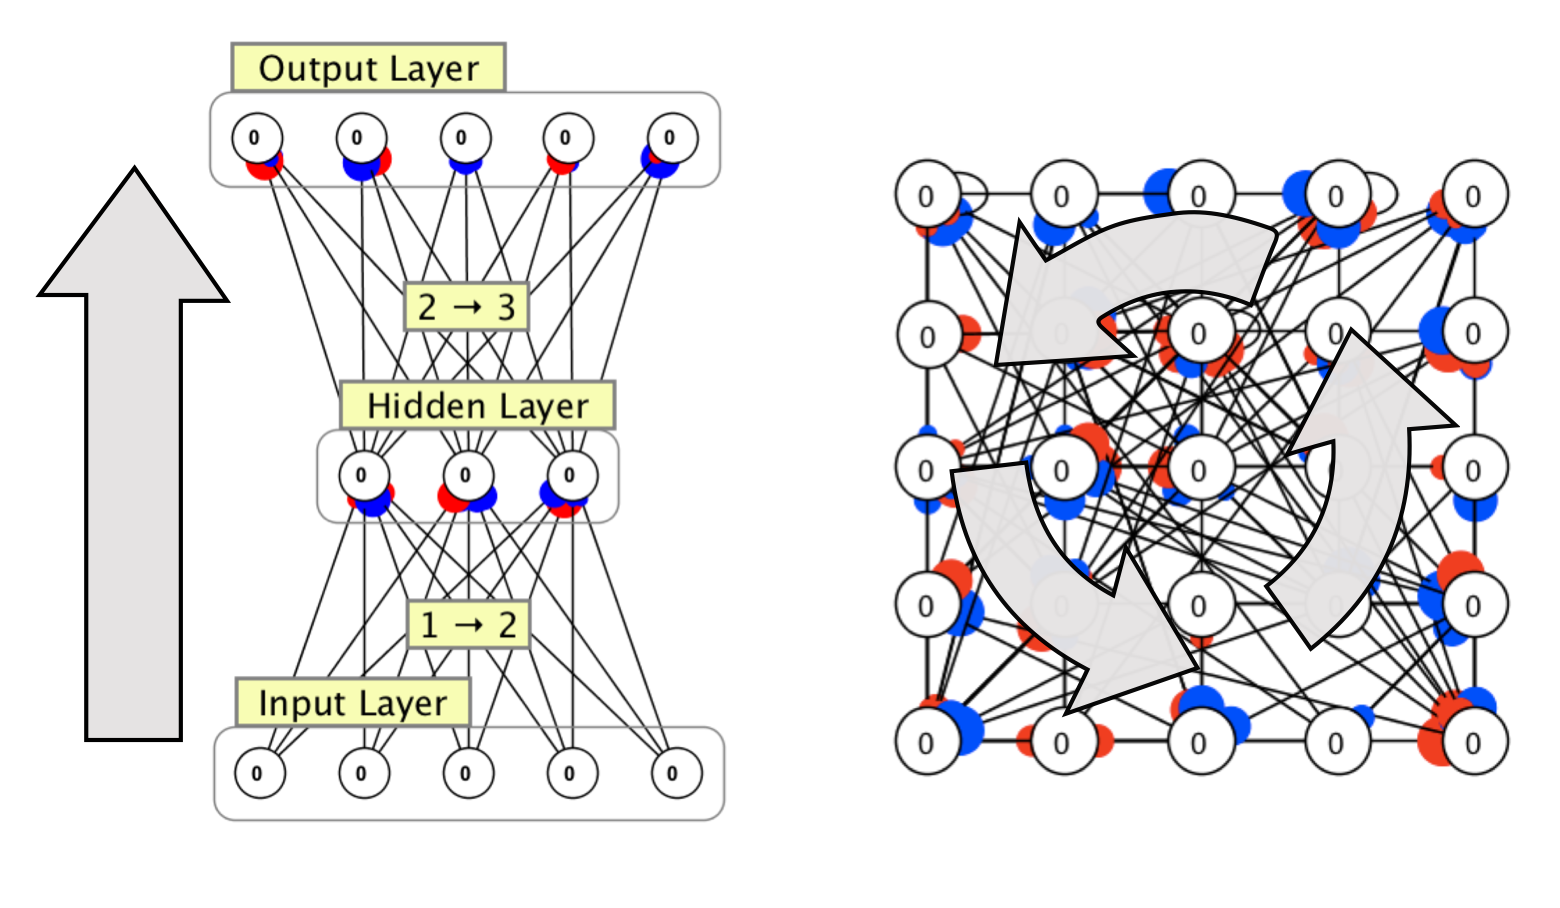
\includegraphics[scale=.7]{./images/NeuralNetTypes.png}
\caption[Simbrain screenshots with additional elements added by Pamela Payne.]{Feed-forward network (left) and recurrent network (right). Gray arrows give a sense of how activation flows through them. The feed--forward network has 3 node layers (a representational ``depth'' of 3, which is not deep; this is not a ``deep network''), and the layers have representational ``widths'' of 5, 3, and 5. }
\label{nn_types}
\end{figure}

%The effects of any input to the network on the network will be completely erased after $n$ iterations where $n$ is the number of layers.
% The graph representing weights from one layer to layer to the next in a feed-forward network is an example of a bipartite graph.

In a \glossary{recurrent network}, the nodes are interconnected in such a way that activity can flow in repeating cycles.\footnote{In graph-theoretic terms, this is a cyclic graph, which contains at least one cycle. Recall from footnote \ref{acyclic} that a directed cycle is a sequence of directed edges that begin and end at the same vertex. That is, starting at one node of such a network, we can ``travel'' from one node to another via the connections and end up back where we started.} Recurrent networks display complex dynamical behaviors that don't occur in feed-forward networks since activity in the network cannot always ``leave'' the network. Most biological neural networks are recurrent. In machine learning, recurrent networks can be used to simulate dynamical processes, for example,  to mimic human speech, or create artificial music.
% Forward ref to DST for a way to study and visualize these
% Any input to such a network \emph{influences} rather than dictates the network's future states, which are determined by both the current input and the current state of the network (itself a product of previous inputs and/or the network's own internal dynamics). 

\begin{figure}[h]
\centering
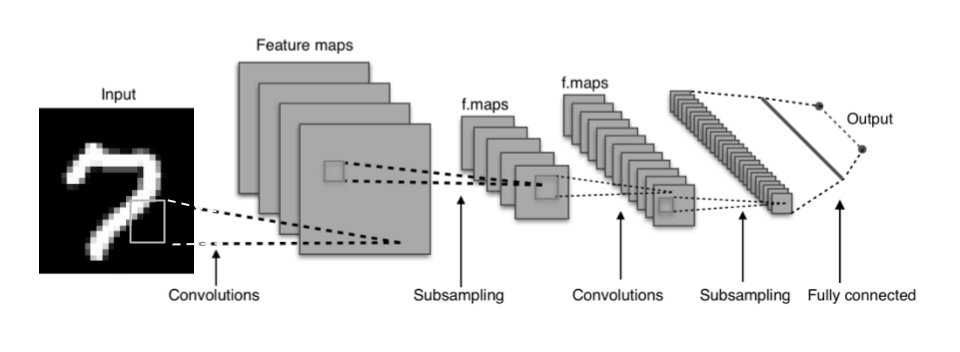
\includegraphics[scale=.45]{./images/deepNet.png}
\caption[Adapted from a creative commons image by Aphex34 at \url{https://commons.wikimedia.org/wiki/File:Typical_cnn.png} ]{A deep neural network, trained to recognize images. The convolutional layers scan over the inputs they are linked to. }
\label{deep_net}
\end{figure}

% Tensor glossary entry. By convention tensor is rank 3 (or more? and used for nodes. Check this. Each sub matrix is  features maps.  
% Each convolutional layer is associated with a fixed set  of weights that is shared. These do different things. Their results are added together. TODO: Fix the picture so it is clear that each 2d node array in each node tensor is associated with a separate convolutional weight layer, which scans across the input.

% History ref
The distinction between feedforward and recurrent networks is a useful first pass way to organize the field. However, more complex architectures are possible, and since the 2010s two specific architectures have been especially common: convolutional networks and transformers.  There is not space to go into these structures here, but we discussion them in chapters \extref{ch_cnn} and \extref{ch_transformers}. These networks operate on data structures more complex than arrays of numbers, for example on 3d arrays or volumes of numbers, which are a kind of tensor (tensors are discussion in section \extref{sect_tensors}). An example of a convolutional network is shown in figure \ref{deep_net}. Networks like this are so large that we can't represent each node and weight separately, and the concept of a layer becomes more complex as more structure and processing is packed into each layer. But the basic concepts of feedforward and recurrent networks that structure the first part of this book still are useful for understanding these more complex developments. 

\begin{figure}[h]
\centering
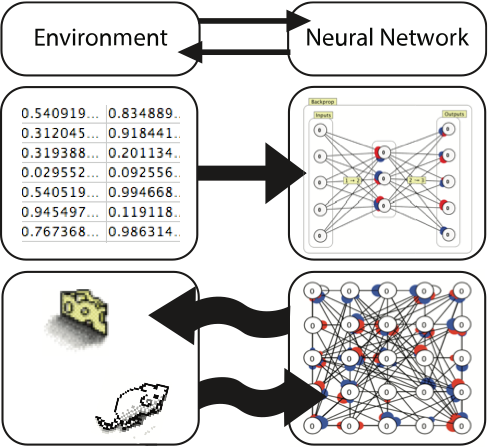
\includegraphics[scale=.7]{./images/nn_environment.png}
\caption[Pamela Payne.]{The relationship between a neural network and an environment. An ``environment'' is often something as simple as a table of values (middle row). However it can also be something more complex, like a virtual world (bottom row).}
\label{nn_environment}
\end{figure}

% Forward ref on RL
Networks almost always exist in some kind of  \glossary{environment}, which gathers inputs for a network and receives its outputs. In cognitive science, the environment of our brain's neural network is the literal environment around us. In some simulations--for example, reinforcement learning simulations--simulated environments are used for neural networks. But if we take environment in a broader sense to simply be whatever it is that produces inputs to an artificial neural network and whatever deals with the outputs, then we capture a broader range of cases.\footnote{Here again we are using ``environment'' in a technical sense that does not track all standard usage, but that is useful for organizing the material and that also draws helpful conceptual connections.}  For example, a neural network that converts speech to text can be connected to audio sensors, like the microphone on your phone. It can take audio in, convert it to text, and send the result out via the speakers. By far the most common way a neural network is linked to inputs and outputs, especially when building and testing them, is via tables of data. Training and testing datasets are discussed at length in chapter \extref{ch_data_science}. In Simbrain, we will also link neural networks to virtual environments. Figure \ref{nn_environment} shows how some of these configurations might look. Couplings between a network and an environment occur at special nodes:  an \glossary{input node}  is influenced by the environment, while an  \glossary{output node} exerts an influence on the environment. In figure \ref{nn_types} (left), for example, the input nodes are the nodes in the input layer, and the output nodes are the nodes in the output layer.\footnote{Information on how to couple nodes to an environment in a Simbrain simulation, and thus treat them as input or output nodes, is available here: \url{http://www.simbrain.net/Documentation/docs/Pages/Workspace/Couplings.html}.} 
%The recurrent network on the right might also have input and output nodes (or nodes that are both at once), but this is not directly visible in that figure.

\section{Computation in Neural Networks}\label{intro_comp_nn}

We've seen what the parts of a neural network are, and learned some basic concepts relating to their structure. We now turn to a few concrete examples in Simbrain that give a sense of how computation works in neural networks. We first develop a basic intuition for how they channel information, and then contrast this with computation in a classical computational system.

\subsection{Basic intuitions: performance and learning}

To develop an intuition for how neural networks ``channel information'' we can break the issue into two parts: performance and learning. 
 
To discuss \glossary{performance}, we consider a network that has already been trained and ask how different inputs propagate through it. That is, we don't change its weights but only change its inputs to see how it responds, given its weights. When you use ChatGPT, you are using a network whose weights have already been set. You are using the final product of a long training process. You write text prompts, they propagate through a bunch of nodes, and new words are generated, one word at a time.  When you talk to a grown person, something similar is happening. They are not learning (much) over the course of a few seconds, but their internal networks are reacting to what you say.  How does this work? At a very basic level, it's simple math. Consider the network shown in the left panel of figure \ref{2NodeSimpleFF}: it's a simple feed-forward network with two input nodes and one output node. The output node's activation is obtained by multiplying each input activation by the strength of the intervening weight; activations are weighted sums of incoming activations.\footnote{This is an example of a linear activation function. The output is See chapter \extref{ch_act_functions}. Often the weighted sum is transformed or processed in further ways. For example, by default in Simbrain nodes have upper and lower bounds that will truncate  activations larger than 1 or less than -1. You can double click on a node to adjust these bounds.}  The inputs are \glossary{clamped node}s, and are represented with a bold outline. This means they will not change their value when we update the network, unless we manually update them.\footnote{If we don't clamp them, then when we update the network they will immediately go to zero, because they have no environment; there are no inputs to them.} Both weights are set to $1$, and so the output is  $.5 \times 1 + .2 \times 1$, or just $.5+.2$. In this case, the output is just the sum of the inputs.  If you have built this network in Simbrain (which is quite easy to do), try pressing the play button and adjusting the inputs up and down to see how this works. It's just adding the inputs together. What could be easier?  At bottom, the same thing is happening even in a giant neural network: each node is taking a weighted sum of its inputs and in this way activation propagates through the network.

\begin{figure}[h]
\centering
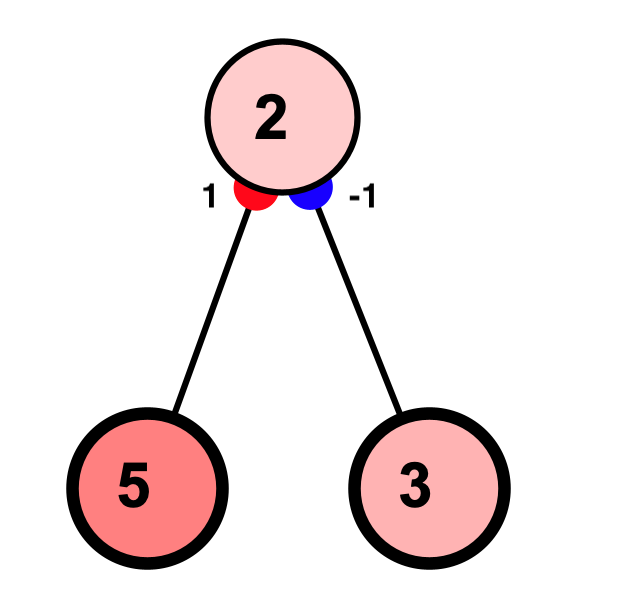
\includegraphics[scale=.25]{./images/2NodeSimpleFF.png}
\caption[Simbrain screenshot.]{Two versions of a simple feed-forward network with clamped inputs. These are linear nodes that simply take a weighted sum of inputs.  In the left panel the weight strengths are both $1$ so the output is $.5 \times 1 + .2 \times 1 = .5+.2 = .7$. In the right panel the weight strengths are $.8$ and $-.1$ so the output is $.8 \times 1 + -.1 \times 1 = .8 - .1 = .7$. By adjusting the inputs or weight strengths, we can make the output activation be whatever we want within the upper and lower bounds of a node. }
\label{2NodeSimpleFF}
\end{figure}

What do we do when a network does not perform as we want it to? We change its weights and other parameters. That is \glossary{learning}. To get a feel for this, we can return to our simple network, set both input activations to $1$ and adjust the weights, to see how how this changes the way information flows through it. In the right panel of figure \ref{2NodeSimpleFF} the weight strengths are $.8$ and $-.1$, and so the output is $1 \times .8 + 1 \times (-.1) = .8 - .1 = .7$. You can recreate this by clicking on the weights and using the up and down buttons, or double clicking them to set them directly.\footnote{Note that we ignore negative activations for now. This is not completely unrealistic. In fact, in some contexts negative activations are taken to be unrealistic or problematic. Neuron spiking rates are always positive, for example. In recent years the ``relu'' activation function, which disallows negative activations, has become extremely popular in deep learning.} Given that both inputs are positive, we can think of positive weights as enhancing inputs and negative weights as diminishing inputs. That is, in this case:
\begin{enumerate}
\item  Positive weights (red disks) increase or excite outputs. They ``heat things up.'' As they are strengthened, the output gets larger.
\item  Negative weights (blue disks) decrease or inhibit outputs. They ``cool things down.'' As they are strengthened (as their absolute value is increased), the output gets smaller.
\end{enumerate}
The two weights are like two knobs that we can turn up or down, that we can use to \emph{tune} the network's response to a set of inputs. Suppose we want the output to be some other value besides $.7$, like $.9$. To do this, we could strengthen the positive weight a little bit so that it makes the output larger. To reduce the output to $.5$, we could  strengthen the negative weight so that it inhibits the output more.\footnote{In the first case, we could also weaken the negative weight so that it inhibits the output less. In the second case, we could also weaken the positive weight so it excites the output less.} With these two knobs we can get the network to do pretty much whatever we want.  Most of the theory of neural networks is about automatically tuning the weights and other parameters of a network--often many thousands, millions, or more of them--to get them to channel information in a useful way.

As an example, consider the simulation  {\em threeObjectsDist.zip}.  A screen shot of the network, which we call the ``three object detector'',  is shown in Fig. \ref{3ObjectClassifier}.\footnote{A video about the three object detector (including information about how to load it) is available at \url{https://youtu.be/yYzUmcPaurI?t=380}. } The three object detector has a feed-forward topology with three nodes in the input layer, seven nodes in the hidden layer, and three nodes in the output layer.\footnote{The example is not meant to model the brain directly. It is more abstract:  it classifies inputs in a  brain-\emph{like} way. It takes a pattern of inputs, and transforms those inputs through a network of connections. This is similar to the way information processing occurs in the brain. But it is not a realistic simulation of a brain circuit (as we will see, it is a ``connectionist network'' as opposed to a ``computational neuroscience'' model; it is also similar to how computations are done in engineering applications).}In this example we also see how a network can be linked to a virtual environment. The mouse on the right of figure \ref{3ObjectClassifier} is hooked up to this network. When the mouse is moved around, the activation in the input nodes changes. This simulates the way odor molecules impact the inner lining of the nose, causing sensory neurons to fire at different levels. So the input layer is a kind of simulated nose. 
\begin{figure}[h]
\centering
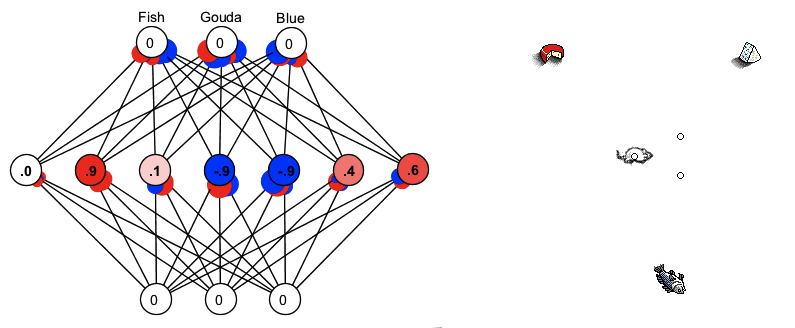
\includegraphics[scale=.4]{./images/3Node_World.png}
\caption[Simbrain screenshot.]{Simple feed-forward network that recognizes three objects.}
\label{3ObjectClassifier}
\end{figure}
% Possibly put in Beer Categorical perception picture here for an example of mixed

Let's first consider its performance. Press play and move the mouse around. (As you do, the weights are not changing). When we move the mouse close to an object, the corresponding output responds.  When we move it away, it decays back to zero.  This is called a \glossary{classification task}. It is performing well.  It responds to each object by activating the appropriate node and no other.

However, this did not just happen by luck. We had to train the network. To see this, try pressing \texttt{w} and then \texttt{r}, to randomize all the weights. That more or less destroys what it has learned. Now press play and move the mouse around again. It can no longer classify inputs. But if you double click the interaction box labeled \texttt{Backprop} and hit the play button in the resulting diaolog, it quickly learns to perform the classification task again. Error drops to zero, and it does what we want. This shows on a small scale how most neural networks are trained.

\subsection{Comparison with classical computation}

% TODO: Add a discussion of AI here and how the term "AI" has changed. Classically it refers to this kind of contrast case.  The point is currently in the first footnote but a bit more historical context could be added here.

We can use the 3-object detector to illustrate certain  general properties of computation in neural networks, which can be contrasted with classical computation in a digital computer.\footnote{Of course, neural network simulations are usually run on a traditional computer performing classical computations. But that is a convenient way of implementing the formal structure of a neural network. These implementation can still take advantage of all the special properties of neural networks. Moreover, it is in fact possible to implement neural networks directly on hardware.} In a classical computer discrete symbols (comprised of strings of 0s and 1s, or ``bits'') are operated on by rules, in a sequential manner. Bits of information are placed in registers on a computer's central processing unit (CPU), and logical rules in the CPU's instruction set are applied to these bits. Computers are hand-programmed to do useful things. The inside of a CPU and the memory systems on a computer are carefully controlled environments. They do not do well with noisy signals or damage. Computation in a neural network is  different. Neural computation is not based on sequential, rule-based operations on bits, but on parallel operations where patterns of node activations are transformed by weight strengths.\footnote{We can often represent this as a transformation of \emph{activation vectors} (lists of activation values) by \emph{weight matrices} (tables representing weight strengths). So, while the basic formalism of classical computation is logic,  the basic formalism of neural networks is \emph{linear algebra}, which we study in chapter \extref{ch_linear_algebra}.}    Neural networks are also more tolerant of noisy signals and damage than digital computers are. Moreover, they are not programmed, in the way a computer is, but are trained, in something like the way a human child is.

Let's use the three object detector simulation to consider some of these contrasts in more detail. 

Networks are \emph{trained} via \glossary{learning}, not programmed. We show the network what we want it to do, and it learns to do it. In the three object detector, for example, here is (very roughly) what happened: we put the mouse near the fish, and said, ``when you smell something like this, fire your first node.''  Then we did the same thing with the Gouda and blue cheese. Each time we exposed the network to an object, we used the ``backprop'' algorithm (discussed in a chapter \extref{ch_supervised}) to adjust the network's weights. At first the network made mistakes, but with each exposure to an object the weights were changed a little, and over time it got better and better at recognizing cheese, in something like the way humans and animals gradually get better at doing things with training. This is called \glossary{supervised learning}, since we know the correct output for each input and can tell the network exactly what output it should produce for any given input.  The great thing about this is that once we've trained the network on some data, \glossary{generalization} is possible, where it can deal with new data it's never been exposed to before. We can train a network to respond to a bunch of cheese we have available, and on that basis it can recognize new pieces of cheese it's never seen before. This is part of what makes neural networks--both the one's used in your cell phones but also the one that is inside your skull right now helping you read this--so valuable. After a bit of training and learning, they can be let loose in the world and deal with brand new situations.

This isn't the only way neural networks can be trained. For example, neural networks can also learn by a system of rewards and punishments (reinforcement learning). They can also learn without any kind of training signal or reinforcement, simply by picking up on the statistical structure of their environment (\glossary{unsupervised learning}).\footnote{Much more rarely, the weights are hand-crafted, as in the IAC networks later in this chapter. But that is the exception that proves the rule. IAC networks are great at illustrating activation dynamics, but highly unusual in that the weight strengths are not learned from data, but are hand-set by a human.}

Second, neural networks emphasize \glossary{parallel processing}. Whereas digital computers normally do things one at a time, in a sequence, neural networks do a lot of things  \emph{at the same time}. To see the difference this can make, consider a simple problem: finding which of ten cups has a jelly bean under it. A serial approach would lift each cup up, one at a time, until the jelly bean was found. A parallel approach would lift all ten cups up at once. Neural networks operate like this, processing information in all the nodes, all at once, all the time. This is easy to see  in the three object detector simulation: when you run the simulation and drag the mouse around, the activations of all the nodes will change based on the new inputs in parallel.\footnote{Of course, you run Simbrain on a conventional computer, so that in reality, the neural network is updated in serial. But this is just an artifact for convenience. In our brains, neurons fire in parallel, and large scale simulations of neural networks are also run in parallel (often on massive distributed computing clusters). In fact, all of the advances in the field since 2010 require parallel computation to achieve the required performance.} 

% Do a pass on the footnote below before re-introducing it
%\footnote{Parallel computation is clearly faster. So, why not do everything in parallel? The answer, roughly, is that the whole theory of digital computation assumes a core level of serial processing. To implement a basic algorithm assumes that things happen in a well-ordered fashion. Techniques for parallel computation exist, and are emerging as an important area of computer science, but in those cases tasks are merely broken down into sub-tasks which are each run in serial side-by-side. However not every algorithm is ammenable to this sort of decomposition (many tasks require the full evaulation of some portion of the task before another step in the task can be started) and to make matters worse the physical limitations of computer hardware as it pertains to memory management and allocation prevents even those which are ammenable from achieving peak theoretical performance. With a few (rare) exceptions 8 processing elements (PEs) working on a task in parallel will never complete a task 8x faster than a single PE for these reasons. However this sort of parallelism isn't the same kind of parallelism as what we find in living neural networks. In computer-world we have synchronous, discrete parallelism; in neuro-world we have asynchronous, continuous parallelism. A great many neurons act asynchrnously in parallel each as its own mini-PE sending and receiving signals from sensory inputs and other neurons such that what exactly each neuron is responding to or what its doing can be quite nebulous. The sorts of representation of information that the brain can support are fuzzy and fleeting, but robust. This tends to be excellent for recognizing objects, catching a fly-ball, learning to move, making analogies or being creative, but in general is poorly suited to (for instance) fast, accurate, memory-intensive numerical computation. This fuzziness is perfect for our very fuzzy world, but in the realms math and logic can be prone to mistakes. 

 %Moreover, serial computers are fast these days. For example, the computer I'm writing this on performs several billion operations per second. With numbers like those we can tolerate the processing slow-down due to serial processing.On the other hand, massively parallel processors like the brain are messy, they make mistakes. They are not as good as computers at performing, e.g., complex mathematical computations or looking up names in an index. And they are made of relatively slow materials. Neurons fire at most 200 times per second. They are orders of magnitude slower then the transistors on this computer. In order to solve problems in a reasonable time frame the brain operates in parallel: every neuron is always doing its own thing. The trade-off is in accuracy: the brain is a kind of messy computer, which doesn't always do the same thing twice. But given the wet, biological stuff we're made of, it works well enough.}

% More details on what to do in sim
Third, neural networks experience \glossary{graceful degradation} when they are damaged (this is also called ``fault tolerance''). They are not brittle in the way a digital computer is. You can start deleting the weights of a neural network and it will still work reasonably well. You can try doing this on the three object detector!   In a  similar way, if you lose a few neurons and /or synapses, you will be just fine. Of course, if you lose enough neurons and synapses it will start to show, but it will happen gradually and  proportionally to the damage. It is in this sense that neural networks degrade ``gracefully.''\footnote{This is related to the fact that they operate in parallel rather than serial. A neural network has lots of redundant wiring which can compensate for damage.}  A digital computer, by contrast, is not designed to continue functioning if its components are damaged. Pluck a micro-chip out of the motherboard, or snip a few wires, and there's a good chance your computer will stop working altogether.\footnote{A related point is that neural networks are good at \emph{handling noisy inputs}. Digital computers don't like noisy input: they respond only to clean, precise inputs. Anyone who has worked with computers has some understanding of this. To get through a company's phone tree you have to enter just the right sequence of numbers--no mistakes allowed!  But show me the same flower ten times, and I will see it as the same flower, even though the input to my brain is changing slightly (the lighting changes, things in my retina change, the whole process is noisy). You can see this in the Simbrain simulation by dragging the mouse around. Notice that even while the inputs change slightly the network continues to recognize which object it's looking at.}

Fourth, neural networks are well-suited to using \glossary{distributed representation}s, rather than \glossary{localist representation}s. Mental representations (e.g. your knowledge of your grandmother) can be thought of in two ways: as being locally stored in one location in the brain, or as being distributed over many locations. A local representation scheme for the brain is sometimes called a ``grandmother cell'' doctrine, because it implies that there is just one neuron in your brain that represents your grandmother. In the context of neural networks, we can say that an object is locally represented by a neuron when activation of that neuron indicates the presence of that object. For example, in figure \ref{localist}, blue cheese is locally represented by the neuron labelled ``Center 5''. When that neuron is activated, the blue cheese is present (here, ``activation'' means having a non-zero, positive activation value).\footnote{Some older types of neural network use only local representations (e.g. the IAC networks discussed in this chapter), and we will see that it is sometimes useful to use local representations. However, the problem with local representations is that you lose some of the virtues above, in particular graceful degradation. If there is just one unit whose activation represents my grandmother, then if I lose that neuron I lose my whole memory of my grandmother. But the empirical evidence suggests that losing a single neuron will not lead to a person's losing an entire memory. So, even if some artificial neural networks use localist schemes to illustrate certain concepts, biological neural networks don't seem to.}

\begin{figure}[h]
\centering
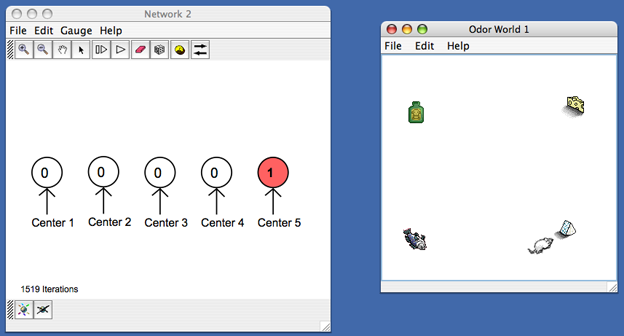
\includegraphics[scale=.3]{./images/Local_Rep.png}
\caption{Localist representation}
\label{localist}
\end{figure}

In contrast, we can say that an object has a distributed representation in a neural network when a particular {\em pattern of activation} over a set of nodes indicates the presence of that object. In figure \ref{distributed},  the bottle of poison has a distributed representation. When the poison is present, a specific pattern of activation $(.1,1,.7,0,.2)$ occurs across the whole set of nodes.

\begin{figure}[h]
\centering
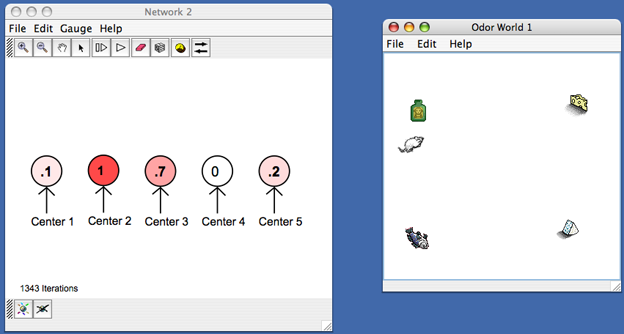
\includegraphics[scale=.3]{./images/Distributed_Rep.png}
\caption{Distributed representation}
\label{distributed}
\end{figure}

For the most part, distributed representations are what one finds in the brain. Generally speaking, brain functions are distributed over many neurons. Although it is harder to think directly about distributed representations than about local representations, a whole conceptual framework has developed which addresses the problem. In fact, much of the book is about developing a mindset that allows you to think about patterns of activation as points in a space (see in particularchapters \extref{ch_linear_algebra} and \extref{ch_dst}).  From that standpoint, the 3 object detector learns how to detect clusters of points, similar ``smells in smell space.'' 

\section{Types of Neural Network Research}\label{typesOfResearch}

% This discussion keeps expanding and so it might warrant a new section or subsection of some kind.
% Rep alignment, interpretability, Zipser. Activation patching. Mechanistic interpretability.
% "Every time I fire a linguist, the performance of our system goes up." Apocryphal to Frederic Jelneck as reported by Sven Matty.  Same for neuroscientist, philosopher, whatever, ML and gradient descent seem to just power their way through any attempt to post hoc understand this stuff.

In practice, neural networks are used in two main ways: (1) as engineering tools, and (2) as scientific models.\footnote{See the discussion of ``standards of intelligence'' in \cite{noelle2022artificial}. Models of idealized intelligence are what we are calling ``engineering'' models here, while psychologically realistic cognitive models are what we are calling ``neural networks as scientific models.''}

When neural networks are used as engineering tools, they are used to do useful things, like recognize faces in photographs or convert speech to text. Neural networks used for engineering do not have to be psychologically or neurally realistic, they just have to work well. In fact, it is preferable if they are \emph{better} than humans, making fewer mistakes than we do.

\begin{figure}[h]
\centering
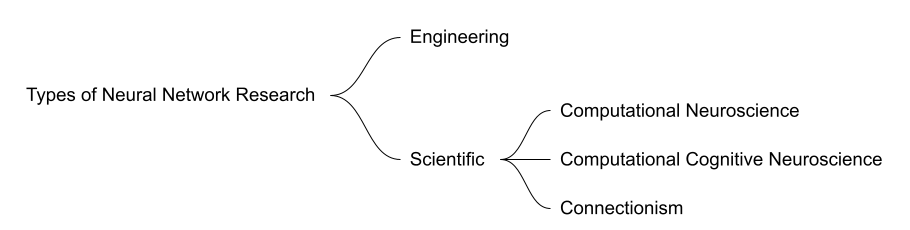
\includegraphics[scale=0.4]{./images/TypesOfNNResearch.png}
\caption[Jeff Yoshimi.]{A taxonomy of types of neural network research, which serves as a guide to this section. Engineering uses (section \ref{machineLearning}) where the goal is to just make something useful, and scientific models where the goal is use neural networks to model the mind (connectionism, section \ref{connectionism}), the brain (computational neuroscience, section \ref{computationalNeuroscience}), or both (computational cognitive neuroscience, section \ref{mixedCases}).}
\label{typesNN}
\end{figure}

Neural networks used for scientific modeling should be neurally or psychologically realistic; they should accurately describe how the brain and the mind work. A neural network model of human memory, for example, should remember (and forget) things in the same way humans do in experiments. This second use of neural networks--as models of the mind and brain--itself subdivides into several subcategories, depending on what specifically is being simulated. Neural networks are sometimes used to understand the brain (in the field of ``computational neuroscience''), sometimes to understand mind and behavior (this is sometimes called ``connectionism''), and sometimes to understand both brain and mind simultaneously. A map of these types of research is in figure \ref{typesNN}. As we will see, this taxonomy is not always so neat, and there are fascinating cases of, for example, engineering neural networks becoming objects of scientific interest.
 
\subsection{Engineering uses of neural networks}\label{machineLearning}

% Other engineering uses: 
% Fausett section 1.3
% Wiki deep  learning page

Neural networks in engineering are tools to solve problems. They are used as classifiers, controllers, signal processors and other components, alongside many other types of engineering tools. In fact, in the contemporary world, many things we take for granted are built on top of neural networks engineered to do useful things. They are at the heart of the current revolution in AI (as of 2023). They recognize voice and images, they generate speech, the generate images and movies, they drive cars, and of course, they can have human-like conversations with us (as with large language models like ChatGPT). They do many of the things humans do, often better than we can, because we can carefully engineer them and train them on such massive datasets.

We will see in later chapters how to systematically classify these different kinds of models, but for now we can focus on a very common case: the use of neural networks to classify objects, which is  one application of  \glossary{machine learning}. Classifiers are good at  finding patterns in complex and noisy data. Remember, neural networks are trained, not programmed, making them well suited to tasks where there is no obvious way to mathematically determine the relationship between a set of inputs and a set of outputs.

% As two workers in the field put it:
%\begin{quote}
%The most natural application areas for [neural networks] are obviously tasks in which appropriate transformations from certain inputs to certain outputs should be established, but the transformations cannot be discovered analytically due to a variety of reasons. Therefore it is no wonder that the most successful applications of the [neural networks] can be found in the areas of machine vision, pattern recognition, motor control, signal processing, etc., where such input to output transformations dominate the problem solving \cite{heikkonen1999building}.
%\end{quote}
%Engineers who use neural networks for these purposes don't care about how the brain works or how humans think: they want to make a machine that works. A neural-network based rice cooker (like the ``Zojirushi neuro-fuzzy rice cooker''; google it!) should make good rice, whether it cooks like humans do or not. 

\begin{figure}[h]
\centering
\raisebox{-0.5\height}{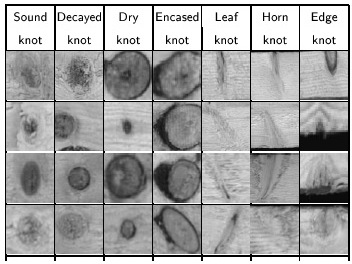
\includegraphics[scale=.4]{./images/wood_network_stimuli.jpg}}
\hspace*{.2in}
\raisebox{-0.5\height}{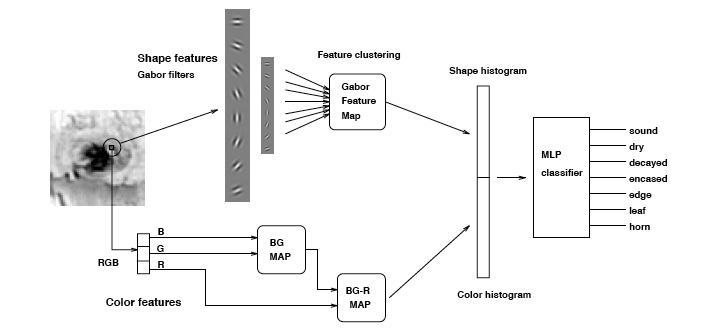
\includegraphics[scale=.3]{./images/wood_network_flowchart.jpg}}
\caption[From Heikkonen et al., 1999 \cite{heikkonen1999building}. Licensed Under CC BY-NC]{Left: Sample inputs to the knot classification network. Right: The knot classification system. The neural network is labelled ``MLP.''}
\label{knotNet}
\end{figure}

Here is an example from the late 1990s. A lumber yard in Finland had to classify pieces of wood, identifying 30 different kinds of knot in images of lumber. Some examples are shown on the left side of figure \ref{knotNet}. A human can classify these knots, but it is time-consuming, expensive, and error-prone (look at how subtle some of the differences are between the different ``dry knots''). It is also hard to program a computer to classify these knots according to explicit rules. Thus, neural networks were used, and they outperformed humans. A neural network trained on samples like the one shown have about 90\% accuracy in this process, compared with 70-80\% accuracy for humans. The neural network is shown in the figure. It is  buried inside the system, the ``MLP classifier'' towards the right (``MLP'' means ``multi-layer-perceptron,'' which is a feed-forward network trained by backpropogation. It is  similar to the 3-object detector above). This system takes a picture of a piece of wood, does some pre-processing on the resulting pixel image, and then summarizes features and colors of that image as a list of numbers, which is fed to the neural network as input. The neural network transforms these numbers into another list of numbers, which describe how decayed, burnt, dry, round, and so forth each sample is. This is a \emph{feature vector}. This feature vector can then be used to classify the knot \cite{heikkonen1999building}.\footnote{Pre-processing is one aspect of data wrangling, which is discussed in chapter \extref{ch_data_science}.  Post-processing also occurs, for example all things that happen in ChatGPT  after the network produces its raw output (for example filtering out inappropriate responses).}
% TODO: Here or above in environment? why here? And make clear processing -> vector -> vector -> post-processing

\subsection{Computational neuroscience}\label{computationalNeuroscience}

We now turn from neural networks used as engineering tools, to neural networks used as models of the mind and brain.

\glossary{Computational neuroscience} uses computational methods to answer questions related to neuroscience. Computational neuroscience spans many levels, from the micro-scale of cell membranes to the macro-scale of the human brain as a whole (see Fig. \ref{compNeuro}). It is a highly multidisciplinary field, encompassing biology, neuroscience, psychopharmacology, cognitive science, complexity science, psychology, and even physics, depending on the context. 

\begin{figure}[h]
\centering
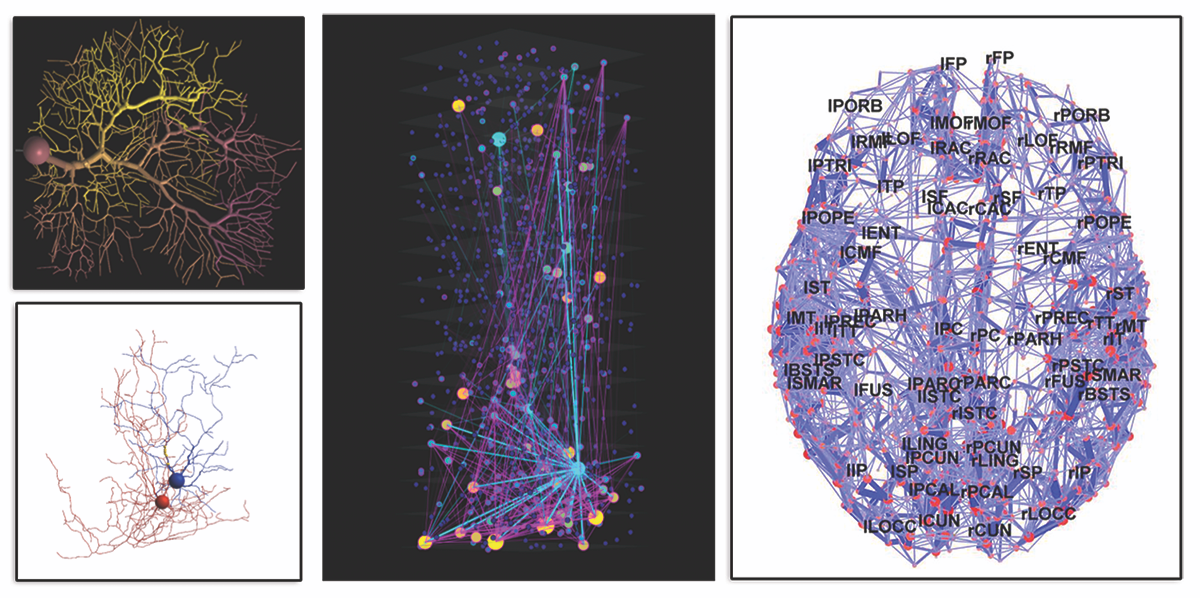
\includegraphics[width=0.8\textwidth]{./images/3typesmodels.png}
\caption[Layout by Pamela Payne. Top Left: ; Bottom Left: ; Middle: Screenshot by Zach Tosi ; Right: From Hagmann et al., 2008 \cite{hagmann2008mapping}, Licensed Under CC BY]{Micro, meso, and macro-level models in computational neuroscience. Left: micro-level models of individual neurons. Middle: meso-level model of a network of several thousand neurons. Right: macro-level model of neuronal connections spread out through the entire brain.}
\label{compNeuro}
\end{figure}
% http://medicalxpress.com/news/2013-11-entire-brain-brainbow-ii-technology.html
% https://upload.wikimedia.org/wikipedia/commons/thumb/e/ef/Network_representation_of_brain_connectivity.JPG/1280px-Network_representation_of_brain_connectivity.JPG

\emph{Micro-scale} models in computational neuroscience study individual neurons or even individual parts of neurons, like the receptors that are studded in the cell membrane to let charged particles in and out of a cell (these are models of ``receptor kinetics''). Models at this level often study the details of how charge flows through the tree-like structures of a neuron's dendrites and axons, and can accurately describe the behavior of individual neurons in a laboratory dish (``in vitro'') when they are injected with current from small electrodes. Models at this level often attempt to answer questions that are physiological or pharmacological in nature like the effect of neuromodulators on the low level dynamics of a neuron, or how new receptors are created or new dendritic spines are grown. These models are largely below the level of what is visible in a single Simbrain node.

\emph{Macro-scale} models in computational neuroscience describe the behavior of large groups of thousands to millions of neurons  and the connections between them. Oftentimes these models approximate the activity of thousands of neurons or even whole brain areas as the activity of a single higher level node.\footnote{As an example, see \url{https://www.ncbi.nlm.nih.gov/pubmed/21511044} \cite{cabral2011role}} These models can accurately describe the spatio-temporal organization of patterns of neural activity measured using brain imaging techniques like fMRI. In a Simbrain network simulation of this kind each node would represent the aggregate activity of thousands to millions of neurons and the whole network could represent the behavior of the entire brain. Models of this type are usually concerned with questions which are psychological or behavioral in nature. For instance the functional relationships between brain regions have been shown to be different in patients with schizophrenia resulting in a different overall graph structure of the functional connectivity between brain regions \cite{bullmore2009complex}. Often work at this level ``bleeds over'' into the realm of general neuroscience.

In this book we mostly focus on the \emph{meso-scale} (or ``middle''-scale) of computational neuroscience, between the micro and macro-levels. Whereas micro-scale models focus on individual neurons or their parts, meso-scale models focus on networks of \emph{hundreds to thousands} (or more) of interconnected neurons. And whereas each node in a macro-level model \emph{approximates} the activity of large group of real neurons, each of the simulated neurons in a meso-level simulation  corresponds to a real neuron. Thus, a meso-level simulation containing 1000 artificial neurons is a direct simulation of a biological neural network containing 1000 real neurons. The emphasis is on discerning governing principles and dynamical phenomena associated with these networks. Meso-level models in computational neuroscience have been implemented in Simbrain (e.g. the middle image in Fig. \ref{compNeuro}). 

The model neurons and synapses used in these simulations  are  more complex than the simple nodes and weights described above in Sect. \ref{structureNets},  since they are designed to mimic the electrochemical properties of real nerve cells. Most neuron models in computational neuroscience are governed by equations acting on variables which represent specific electrochemical attributes of living neurons. Synapses have temporal delays and their signals have duration. Network models in computational neuroscience tend to be comprised of \emph{spiking neurons} (neuron models which produce and propagate signals via action potentials) embedded in complex \emph{recurrent} networks. We cover the special properties of these model neurons and networks in chapter \extref{ch_spiking}.\footnote{In contrast to the micro-scale, which is (broadly) concerned with physiology, and the macro scale, which is often concerned with psychology, the meso-scale concerns itself with questions like: How do networks of interconnected neurons represent information? Can we replicate synaptic connectivity using plasticity rules? How does information processing emerge from the interactions of neurons embedded in a neural network?'  Meso-scale models often attempt to understand formalisms that describe observations of groups of neurons (e.g. slices of brain tissue) with explanations of those observations using models of detailed low level processes at the micro-scale. It is known that when neurons fire in particular temporal sequences the synapses connecting them will become stronger or weaker depending upon that sequence. A micro-scale model might concern itself with how new receptors are created, or new spines are grown. A meso-scale model will only concern itself with the function translating that temporal sequence into a change in synaptic strength.} 

Very roughly, the focus of computational neuroscience at these  three scales can be thought of as follows:
Neuron Dynamics $\rightarrow$ Network Dynamics $\rightarrow$ Brain Dynamics

\subsection{Connectionism}\label{connectionism}

% See Talking Nets 259, 283, 274
% Maybe talk more about semantic memory and semantic network models, and contrast with other types of memory (many will not have taken intro cog-sci courses)
The use of neural networks as cognitive models, which behave in the same way humans and animals do, but without concern for neural realism, is sometimes called \glossary{connectionism}.\footnote{Not everyone using the term ``connectionism'' in this way, but it is a fairly standard usage. A more precise phrase would be ``connectionist model of a cognitive process''.}  In connectionist models, there is no direct effort to understand the brain. The focus is on modeling some aspect of human or animal behavior using nodes and weights. Such models  are usually meant to {\em suggest} how a given task is accomplished by the brain---they are ``neurally plausible''---but they do not directly model the underlying neuroscience.

% Should this be a named section on IAC? Kind of lost in this organization.
% Redo IAC given assignments
% Forward reference to ch_unsupervised_recurrent and DST, it develops fixed point attractors and the transient portion is the thought process
% We have settled on object pool and property pool. Introduce this nomenclature and distinguish it from the original.  Also, use some memory language. Item vs. category retrieval. "exemplars. It can also generalize along an indefinite number of different lines retrieve the specific characteristics of particular exemplars , and fill in plauaible default values for misaing properties."
As an example, consider the ``IAC'' or ``Interactive Activation and Competition'' network. A famous example of an IAC network is McClelland's model of knowledge of two fictional 1950s gangs, the Jets and Sharks from {\em West Side Story} \cite{mcclelland1981retrieving}.\footnote{For a video overview of this network in Simbrain, see \url{https://www.youtube.com/watch?v=Nw3TEDfugLs}.}

\begin{figure}[h]
\centering
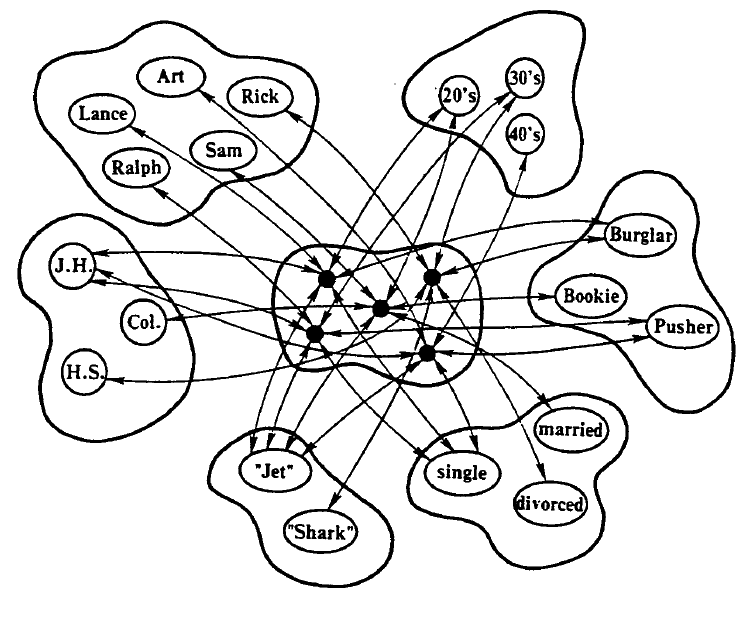
\includegraphics[scale=.3]{./images/IAC_JetsSharks.png}
\caption[From McClelland and Rumelhart, 1989 \cite{mcclelland1989explorations}.]{A fragment of the Jets and Sharks model. Nodes in this model don't represent neural activity, but activation of concepts in semantic memory.}
\label{iac}
\end{figure}

% Maybe just go full Simbrain. Change the example and make clear that it can be done in many ways.
% Make the object pool / property pool distinction more central, and give more examples.
% In a sense a model of the ventral stream, but not the dorsal stream. No ``embodied'' memory captured, no dorsal stream, and no retrieval mechanisms. Maybe refer to publications about actual semantic memory. BUT don't want to emphasize neuro too much so a balance.
% A good contrast to supervised, unsupervised, and generalization. A strange case where we hand-tune the weights. Note there is NO learning in these model. So the concepts of supervised and unsupervised don't apply. It is hand tuned. 

An IAC model is organized into pools of nodes. In Fig. \ref{iac}, there are 7 pools of nodes. These pools of nodes are used to model the internal concepts of a person who knows about these two gangs. The pools represent different  traits:  age, education level, marital status,  job, etc. The central pool is a pool of ``instance nodes'' or ``object nodes'', shown as black disks, which correspond to individual people. Each person is associated with a node. The other pools correspond to properties of these people: their name, job, age, and gang affiliation. The nodes in each pool inhibit each other, which produces a \emph{winner-take-all} structure. As the simulation runs, the activation of one node in each pool will tend to dominate the others. Notice that the topology of this network is recurrent, and as a result the network has dynamics: when we run it, activation starts to spread from one node to another over time. In fact, these have also been called \emph{spreading activation} networks \cite{mcclelland1981retrieving}. 

The IAC network models general features of human semantic memory, like the ability to retrieve attributes of a person based on their name. If the Lance node is activated and the simulation is run, activation will spread through the recurrent network, and after a while the Jets node, 20s node, Junior high education node, and burglar node will have the highest activations. This is like asking ``Tell me about Lance?'' and being told about him. The network can also model our ability to describe the properties of a group of people. If the Jets node is activated and the network is run, the standard characteristics of the Jets will light up: they tend to be in their 20s, with a junior high school education, and single. This is like asking ``Tell me about the Jets?'' and being told about that group. The network can also model our ability to identify people who match a specific description. If the 20s node and the junior-high education node are activated, then the name nodes for Lance, Jim, John, and George all light up. This is like asking ``Who is in their 20s with a junior high education?'' and being told ``Well, that could be Lance, Jim, John, or George.''
%\footnote{Notice that the nodes and connections in this model don't correspond to actual neurons or synapses. The IAC network captures the empiricist theory (associated with John Locke and David Hume) that  human knowledge is encoded in abstract associations between ideas. Node activations correspond to the presence of an item in thought or memory, or what the empiricist philosophers called \emph{ideas}. If the ``Lance'' node is active, that corresponds to a person thinking about Lance. Connections between nodes correspond to \emph{associations} between ideas. The whole network of connections represents our overall knowledge about something, in this case, two gangs. When one node  is activated and the network is run, all the associated nodes are activated. Over time all the ideas associated with the original idea should be activated \cite{mcclelland1981retrieving}. Nodes and weights represent ideas and associations in an abstract brain-like way without modeling neuroscience directly.} \cite{mcclelland1981retrieving}

Though IAC networks are models of semantic memory, and are brain-like (spreading activation and winner-take-all types of dynamics do occur in the brain), they are \emph{not} models of the brain, they do not capture any details of human neuroscience, or have nodes whose activation corresponds to activity in specific parts of the brain.

\begin{figure}[h]
\centering
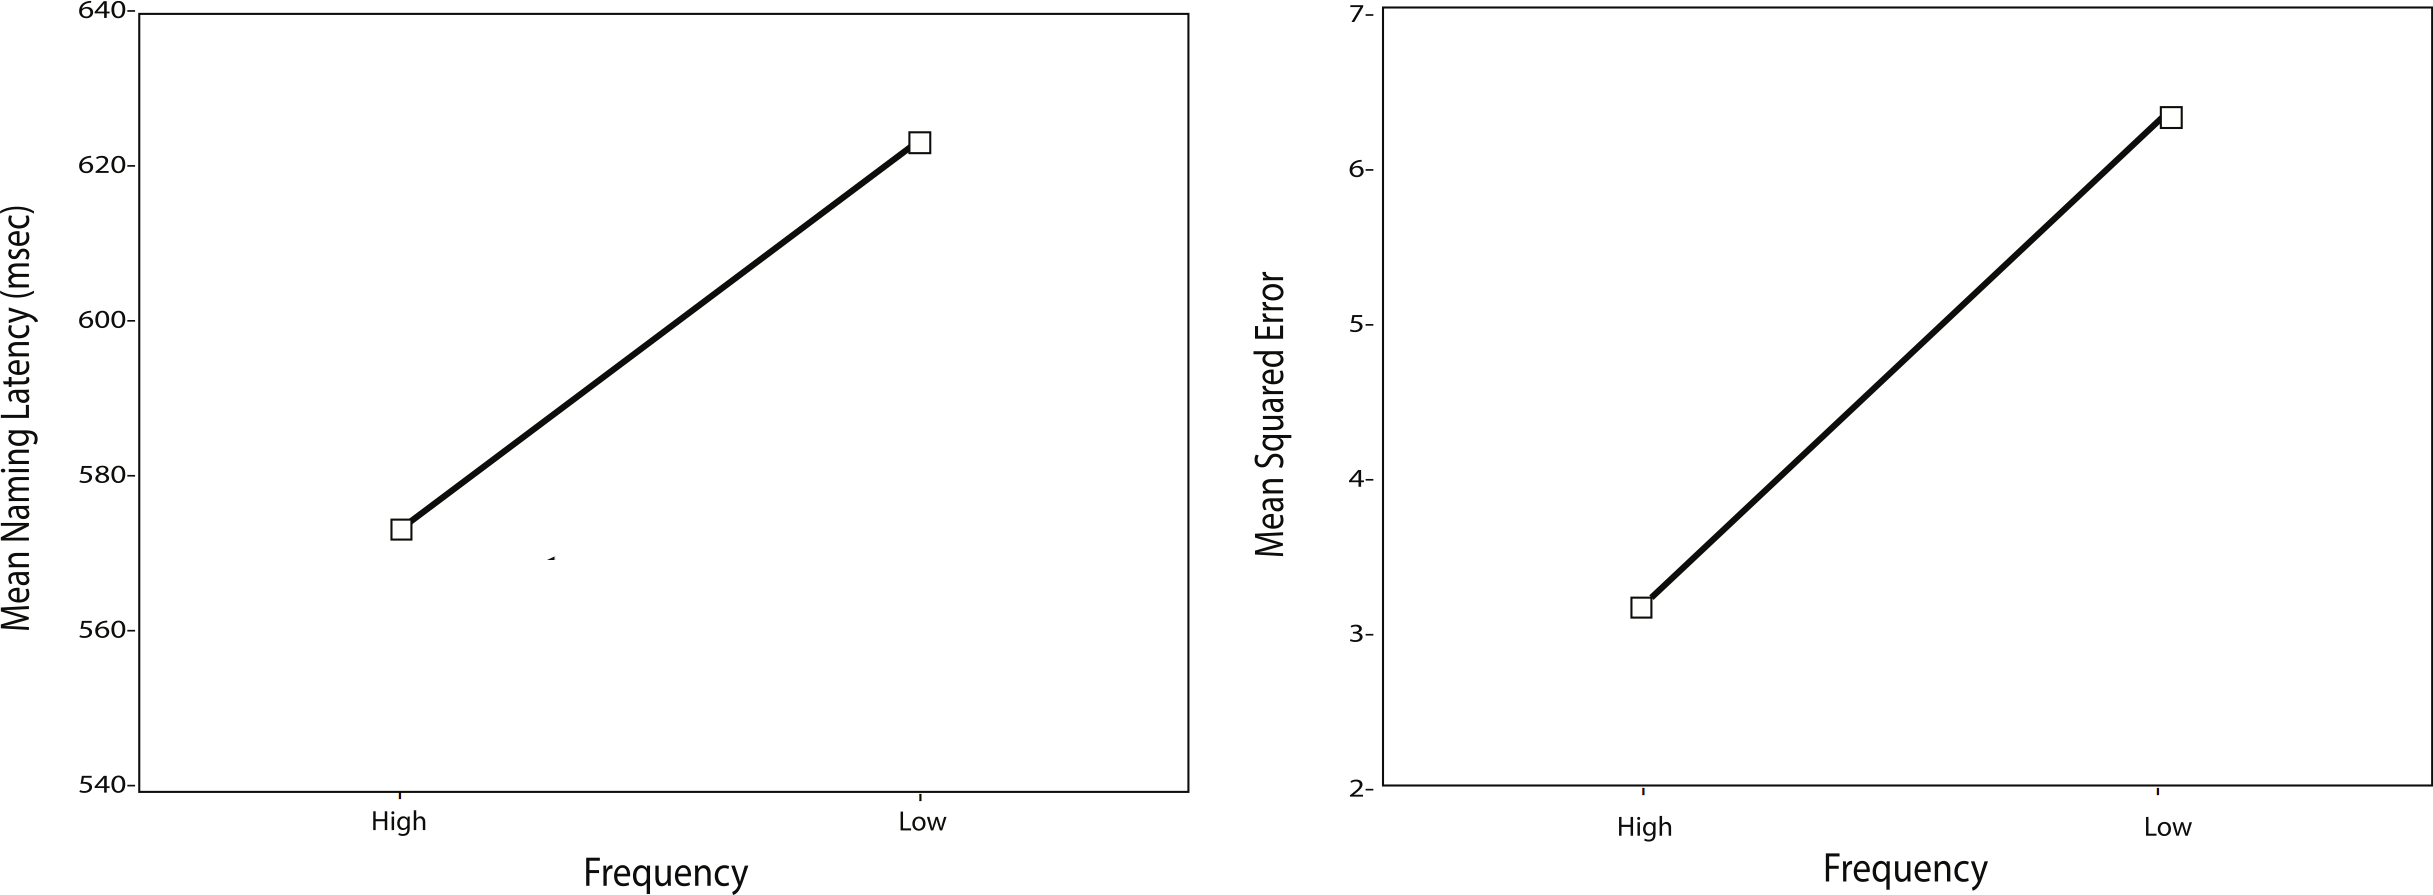
\includegraphics[width=0.8\textwidth]{./images/seidWordNet_Data3.png}
\caption[From McClelland and Seidenberg, 1989 \cite{seidenberg1989distributed}. Redrawn by Pamela Payne.]{Data associated with Seidenberg and McClelland (1989)'s reading model. Human data are on the left, neural network data are on the right. Humans pronounce high frequency words more quickly than low-frequency words. The neural network makes fewer errors on high frequency than low-frequency words.}
\label{regularityData}
\end{figure}
 
% This has become so short it might be time to get remove it, keep things simple. One main example per section. As it is it gets a bit lost. If used, take the opportunity to talk about error in a bit more detail.
The IAC network is a qualitative model of human memory. Other connectionist simulations are more quantitative. For example, Seidenberg and McLelland  modeled childrens' reaction times in reading words aloud. The network is a variant on a feed-forward network, similar to the network on the left side of figure \ref{nn_types}. It has  more nodes: 400 input units, which represent written words, and 460 output units, which represent spoken words. It was trained to pronounce all one-syllable words in English using a method called ``backpropogation'' (chapter \extref{ch_supervised}). This simulation models  the \emph{word frequency effect}. Words that occur frequently in language (like ``the'') are pronounced more quickly than words that occur infrequently (like ``rake'').
%\footnote{\label{exceptionsVsRegular}The model also captures the ``frequency-regularity interaction'', whereby words that have regular pronunciation patterns (e.g. ``gave'' or ``must''), are pronounced faster than exception words (e.g. ``have''  or ``pint''). However, this regularity effect only occurs for infrequent words. This is also shown in the figure: in each graph the upper curve with the open squares show exception words; the lower curves with filled triangles show regular words.}  

Human data showing this effect are on the left side of Fig. \ref{regularityData}. Humans pronounce high frequency words more quickly than  low frequency words (the $y$-axis shows latency, or length of time to pronounce the word; lower values mean faster times). The neural network data on the right  was generated by counting how many mistakes the network made for low and high frequency words \cite{seidenberg1989distributed}. When you line the two graphs up next to each other, they look the same. This suggests that the way the model reads is similar to the way humans read: both the neural network model and humans are better at reading more common words.
%\footnote{ Many questions come up here, and you might not be satisfied (in fact, this model was involved in a kind of war between connectionist and non-connectionist models of  reading). The main thing  to emphasize here is that the model is supposed to capture some kind of human, behavioral data.}

\subsection{Mixed and intermediate cases}\label{mixedCases}

Both distinctions discussed in this section can be difficult to apply. It can be difficult to know whether a neural network model is being used as an engineering or a scientific model, because engineering models end up being used for scientific purposes and vice-versa. In the case of a neural network that is used as a scientific model, it can be hard to say whether it simulates the brain (computational neuroscience), or cognition (connectionism). Many models aim to do both at once.

The first distinction, between engineering and scientific uses of neural networks, can be confusing because the two usages have been historically intertwined. Some neural networks that originated as scientific models later got used as engineering tools. Conversely, sometimes an engineering tool ended up being useful as a scientific model. Deep networks provide a striking example of these back and forths. As we discuss in chapters \extref{ch_history} and  \extref{ch_neuro}, deep neural networks  were originally used as scientific models of vision in the 1970s. These later turned out to be excellent tools for pattern recognition (a common engineering application, for example recognizing digits on an envelope), which led to the deep learning revolution of the 2010s. Then it happened again! These new and improved deep networks turned out to be useful in computational neuroscience as a way to understand the human visual system. So, a neural network that started off in science, then got used for engineering, and then later that tool then got adapted back to science! 

Similar twists and turns from engineering to science are happening now with the emergence of large language models like ChatGPT. They originated as pure engineering models, that are meant to facilitate natural language processing. I think we can all agree that ChatGPT is useful, whether or not it ``thinks like a human.'' But it's so compelling as a model, that linguists, psychologists, and philosophers are starting to study them as cognitive models.  See Chapter \extref{ch_supervised_recurrent}. So in this case a model that started off in engineering subsequently became an object of scientific study.

A good rule of thumb when considering how to classify a neural network is to ask: ``What is the neural network being used for? As a tool, or as a scientific model?''\footnote{A more advanced way to ask this question is to ask: how are the node activations and weight strengths being interpreted? Are they merely parameters in statistical models, or are they supposed to capture something real about neurons, or about concepts and their relations?} Even then it can be tricky. For example, consider the following title of a journal article: ``Use of Neural Networks in Brain SPECT to Diagnose Alzheimer's Disease'' \cite{page1996use}. At first, this sounds like it might be about a computational neuroscience or connectionist model, since it mentions the brain and Alzheimer's. However, the article is actually about how neural networks can be used to determine whether a person has Alzheimer's. The neural network is not being used as a model of the brain or any cognitive processes, but rather as an engineering tool to help diagnose Alzheimer's disease based on brain images. If we ask: ``What is the neural network they made being used for?'', the answer is to build a better diagnostic tool for Alzheimers. The network is \emph{not} being used a model of Alzheimers. So it's really an engineering usage of a neural network, rather than a scientific model.

As far as the distinction within scientific modeling between computational neuroscience and connectionist models, here too there are difficult cases, mainly because many people who use neural network models are interested in \emph{both} how the brain works \emph{and} how cognition works, and of course, how the two are related. Thus, there are increasingly many models that attempt to capture both neural and psychological data, as was noted in the discussion of macro-level computational neuroscience above. 

For example, models in \glossary{computational cognitive neuroscience} attempt to capture psychological and behavioral data while simultaneously paying attention to neural details. This type of model captures various aspects of cognition (e.g. visual attention, semantic and episodic memory, priming, familiarity, and cognitive control), using groups of neurons that are explicitly associated with specific brain circuits. Many researchers hope that over time computer models of brain and behavior will converge, and that future models will increasingly capture both neural and behavioral data, and thereby reveal how the dynamics of the brain give rise to the dynamics of cognition.\footnote{Examples of researchers and research groups working in this area include the work of Randy O'Reilly and his colleagues (\url{https://grey.colorado.edu/CompCogNeuro/index.php/CCNBook/Main}), Stephen Grossberg's work which began in the 1960s (\url{https://en.wikipedia.org/wiki/Stephen_Grossberg}), and the work of Chris Eliasmith and his colleagues (\url{https://uwaterloo.ca/centre-for-theoretical-neuroscience/people-profiles/chris-eliasmith}).} Some examples of this type of model are shown in figure \ref{ccn}.

% Emergent ref since I have a spaun ref?
\begin{figure}[h]
\centering
\raisebox{-0.5\height}{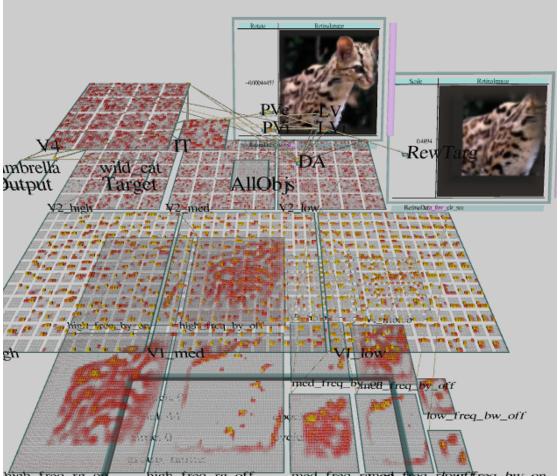
\includegraphics[scale=.3]{./images/EmergentScreenshot.png}}
\hspace*{.4in}
\raisebox{-0.5\height}{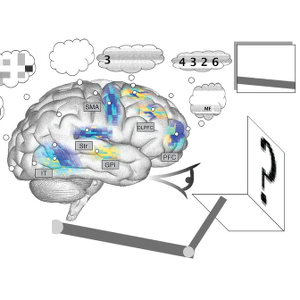
\includegraphics[scale=.6]{./images/spaun.png}}
\caption[Left: From \url{https://grey.colorado.edu/emergent/index.php/File:Screenshot_vision.png}; Right: Spaun screenshot. Cf. \cite{eliasmith2012large}.]{(Left) An Emergent simulation of visual processing, with labels indicating which brain areas each group of nodes represents. (Right) A Nengo simulation of the human ability to retrace a visually perceived number.}
\label{ccn}
\end{figure}

 From this standpoint, computational neuroscience and connectionism are two ends of a continuum or spectrum. We have computational neuroscience at one end, and connectionism at the other. All through the middle of this spectrum are models that try to model both biological data and psychological data at the same time. The goal is to understand how the circuits of the brain produce all the wealth and complexity of observable human and animal behavior. 

% Forward reference to the strange case of BERT